\documentclass{article}

\usepackage{graphicx}
\usepackage[utf8]{inputenc}
\usepackage[T1]{fontenc}

\begin{document}

\title{Predictive Models for Water Demand and Population Growth in the capital area of Iceland}
\author{Sigurdur Haukur Birgisson}

\maketitle

\begin{abstract}
    This research paper presents the development and performance evaluation of predictive models for water demand and population growth in Reykjavik, Iceland. The models utilize data provided by Reykjavik Energy and leverage machine learning algorithms, including XGBoostRegressor and RandomForestRegressor. The study aims to provide valuable insights for resource planning, infrastructure investment, and sustainable development in the water industry. The results demonstrate promising predictive capabilities within the limitations of the available dataset.
\end{abstract}

\section{Introduction}
The water industry plays a crucial role in ensuring sustainable water management practices. Accurate predictions of water demand and population growth are essential for efficient resource allocation and infrastructure planning. This research focuses on developing predictive models to address these challenges in Reykjavik, Iceland.

\section{Data}
The data used in this study was available on Gagnagatt, the open data portal of the Icelandic government, it was collected from Reykjavik Energy (the main company serving water to people in the capital area of Iceland). The hot water \cite{hot-water} and cold water \cite{cold-water}. The datasets contain annual records of water demand, population growth, and related variables. Data from the Icelandic Metiorological Office \cite{weather} was also used.

All the datasets were joined into one, on the year variable. The data was then split into a training set (80\%) and a test set (20\%). The training set was used to train the models and the test set was used to evaluate the performance of the models.

A correlation matrix was created to identify the most important variables. The correlation matrix is shown in Figure \ref{fig:correlation-matrix}.

\begin{figure}[h]
    \centering
    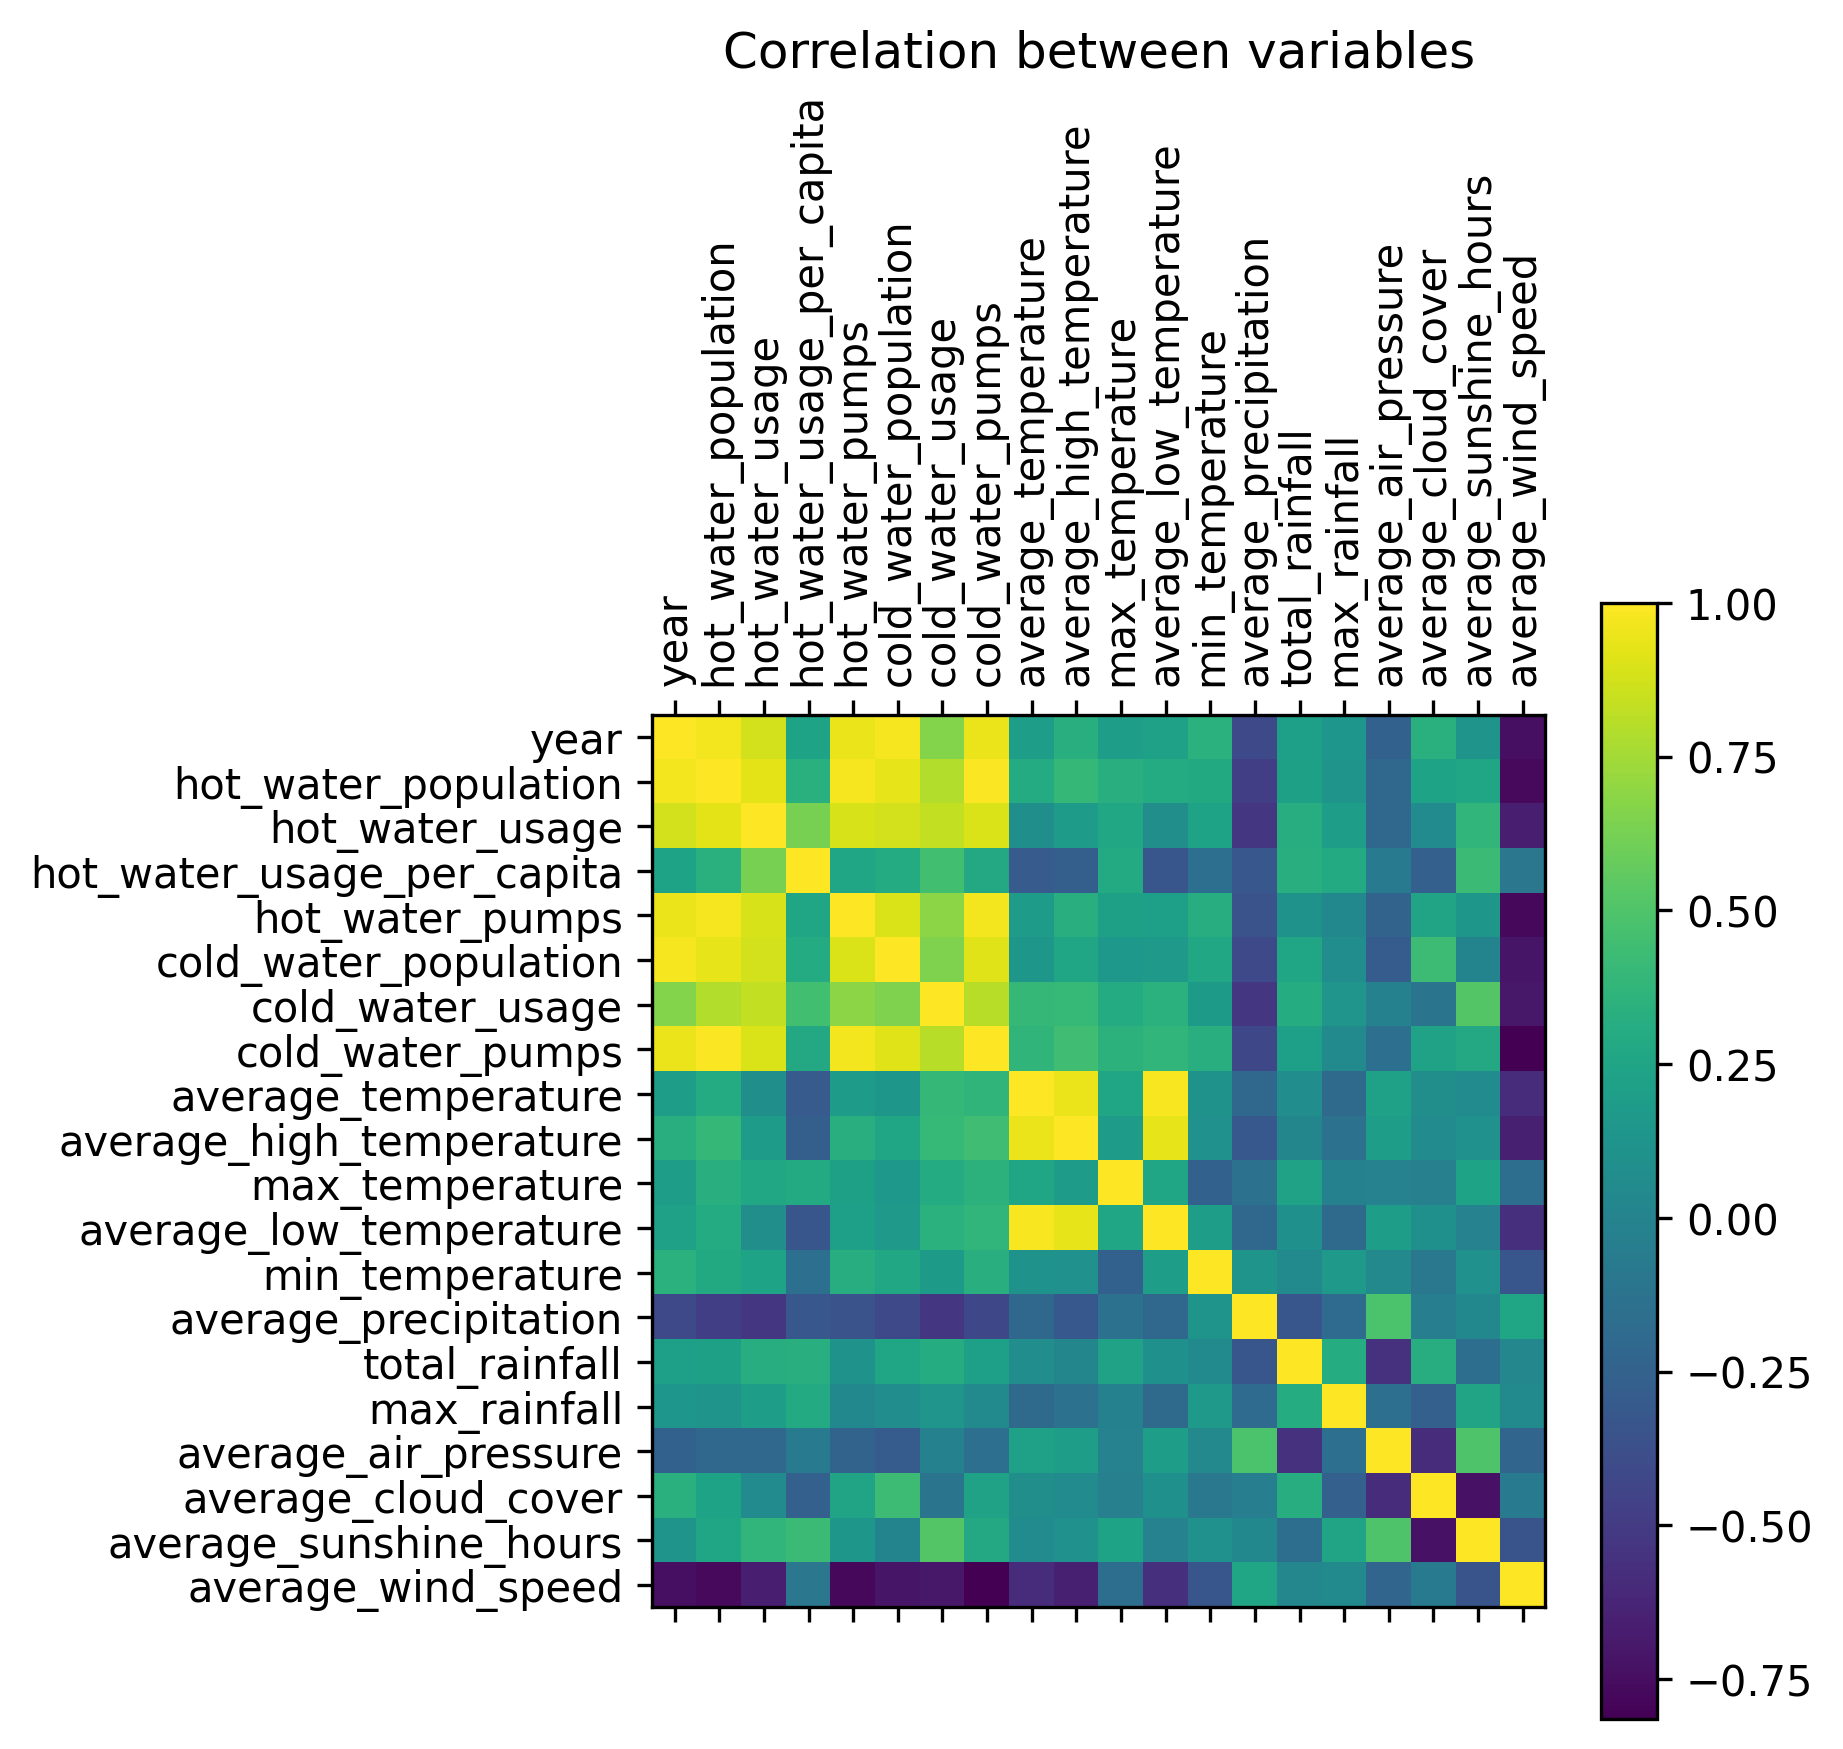
\includegraphics[width=0.8\textwidth]{../figures/correlation.png}
    \caption{Correlation matrix}
    \label{fig:correlation-matrix}
\end{figure}

The correlation matrix shows that the most important variables relating to water demand are the number of people living in the area (e.g. hot\_water\_population), the year (e.g. year), and the average min temperature (e.g. average\_temperature). However the average min temperature has little correlation compared to the other two, so it was not used to predict for water demand.

\section{Methods}
The models were trained on the training set and evaluated on the test set. The performance of the models was evaluated using the mean absolute error (MAE), the root mean squared error (RMSE), and validation accuracy.

Before deciding on the kind of model to use, the trends in the data were analyzed. The trends are shown in Figure \ref{fig:water-demand-trends} and Figure \ref{fig:population-trends}.

\begin{figure}[h]
    \centering
    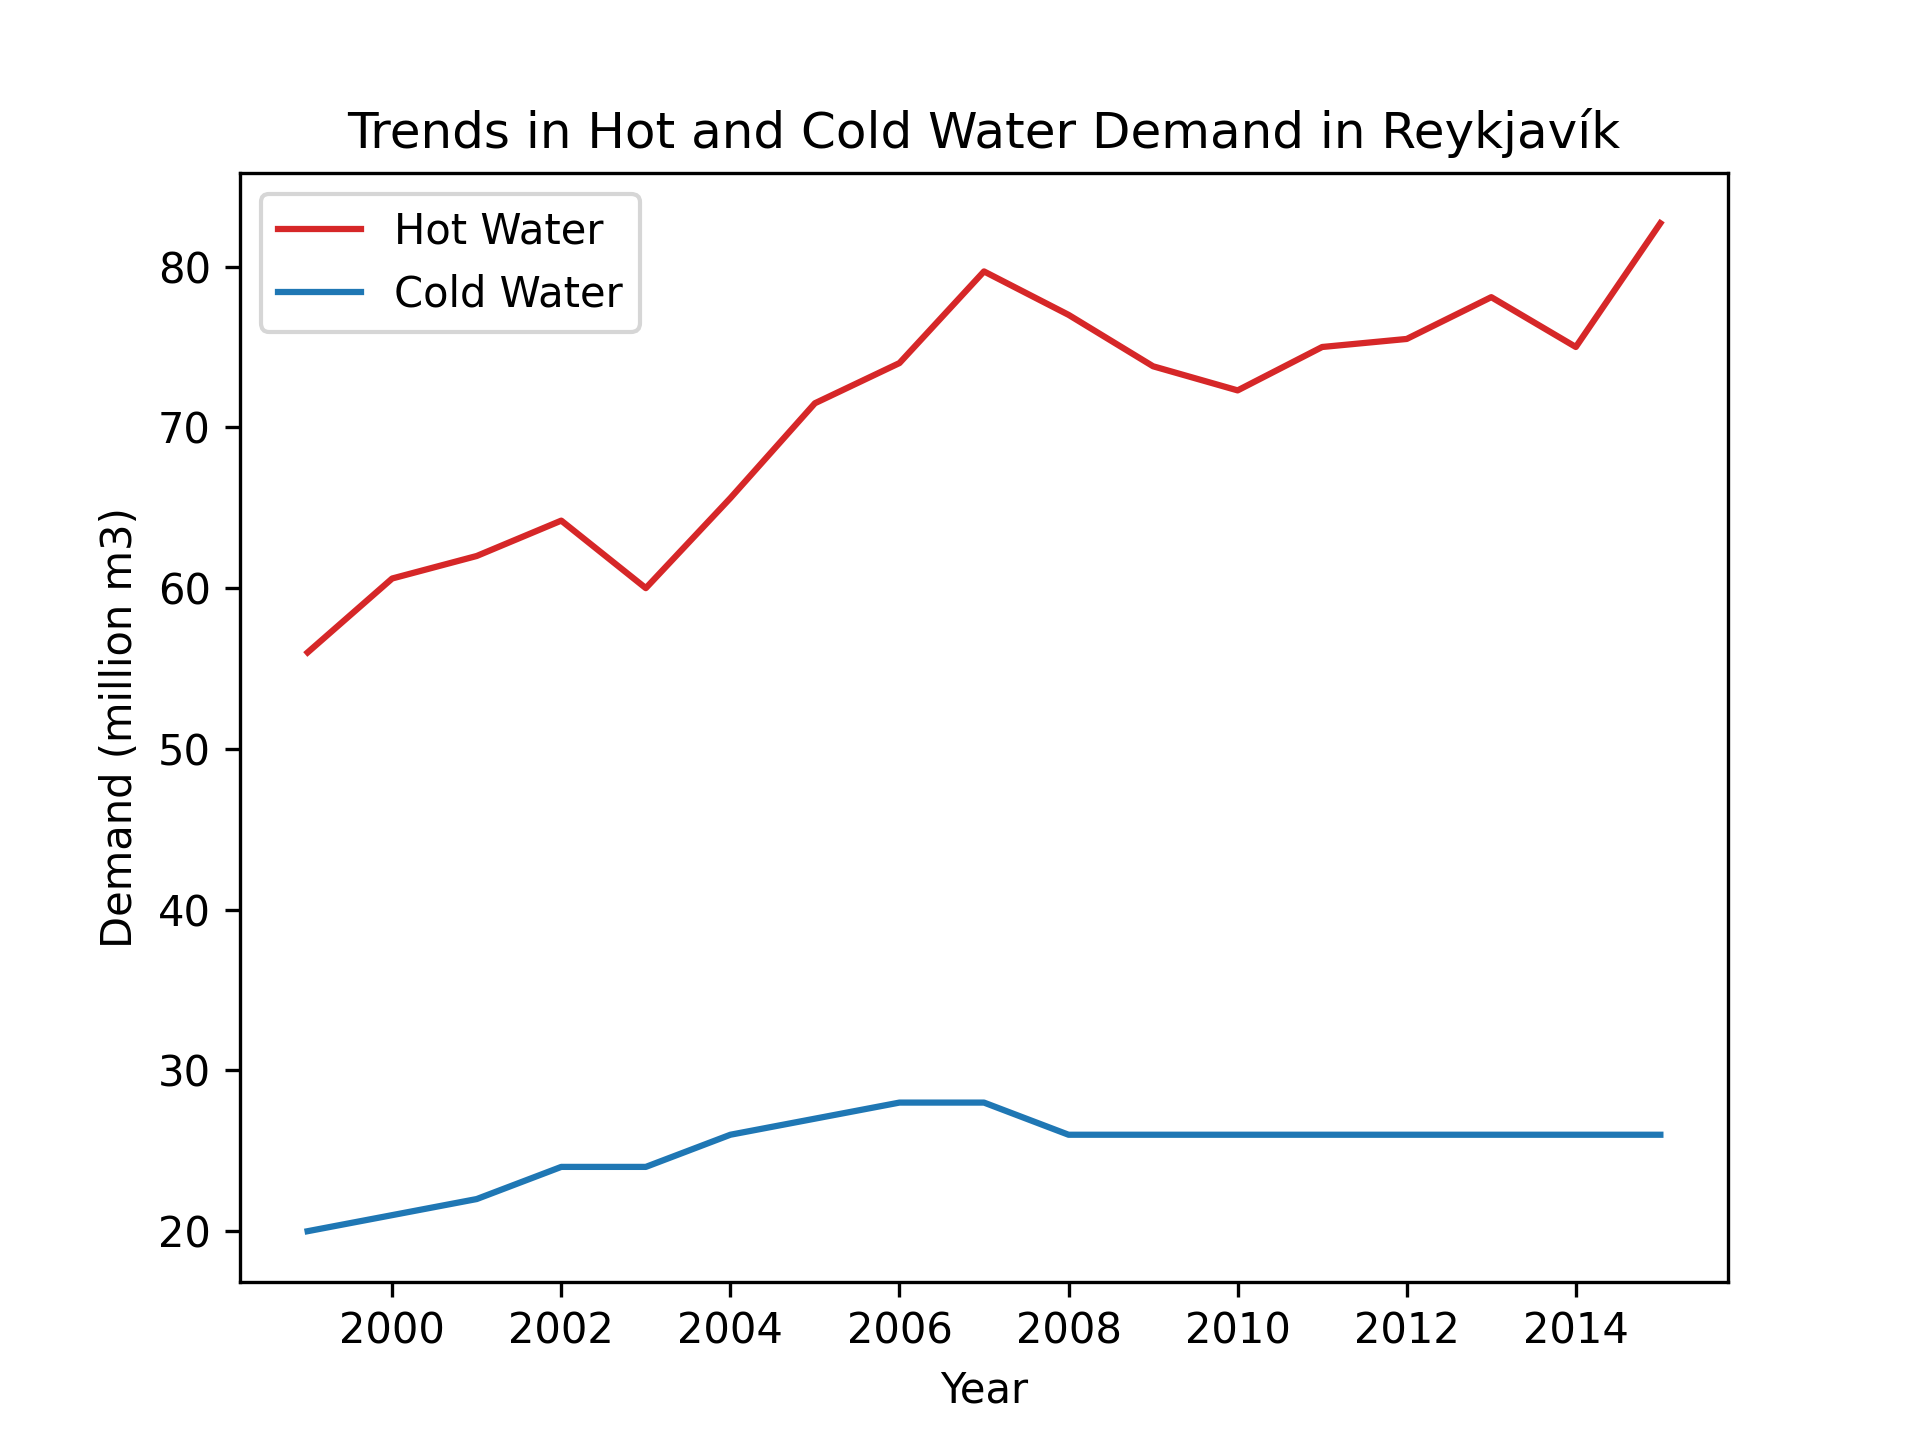
\includegraphics[width=0.8\textwidth]{../figures/trends-in-hot-and-cold-water-demand.png}
    \caption{Water demand trends}
    \label{fig:water-demand-trends}
\end{figure}

\begin{figure}[h]
    \centering
    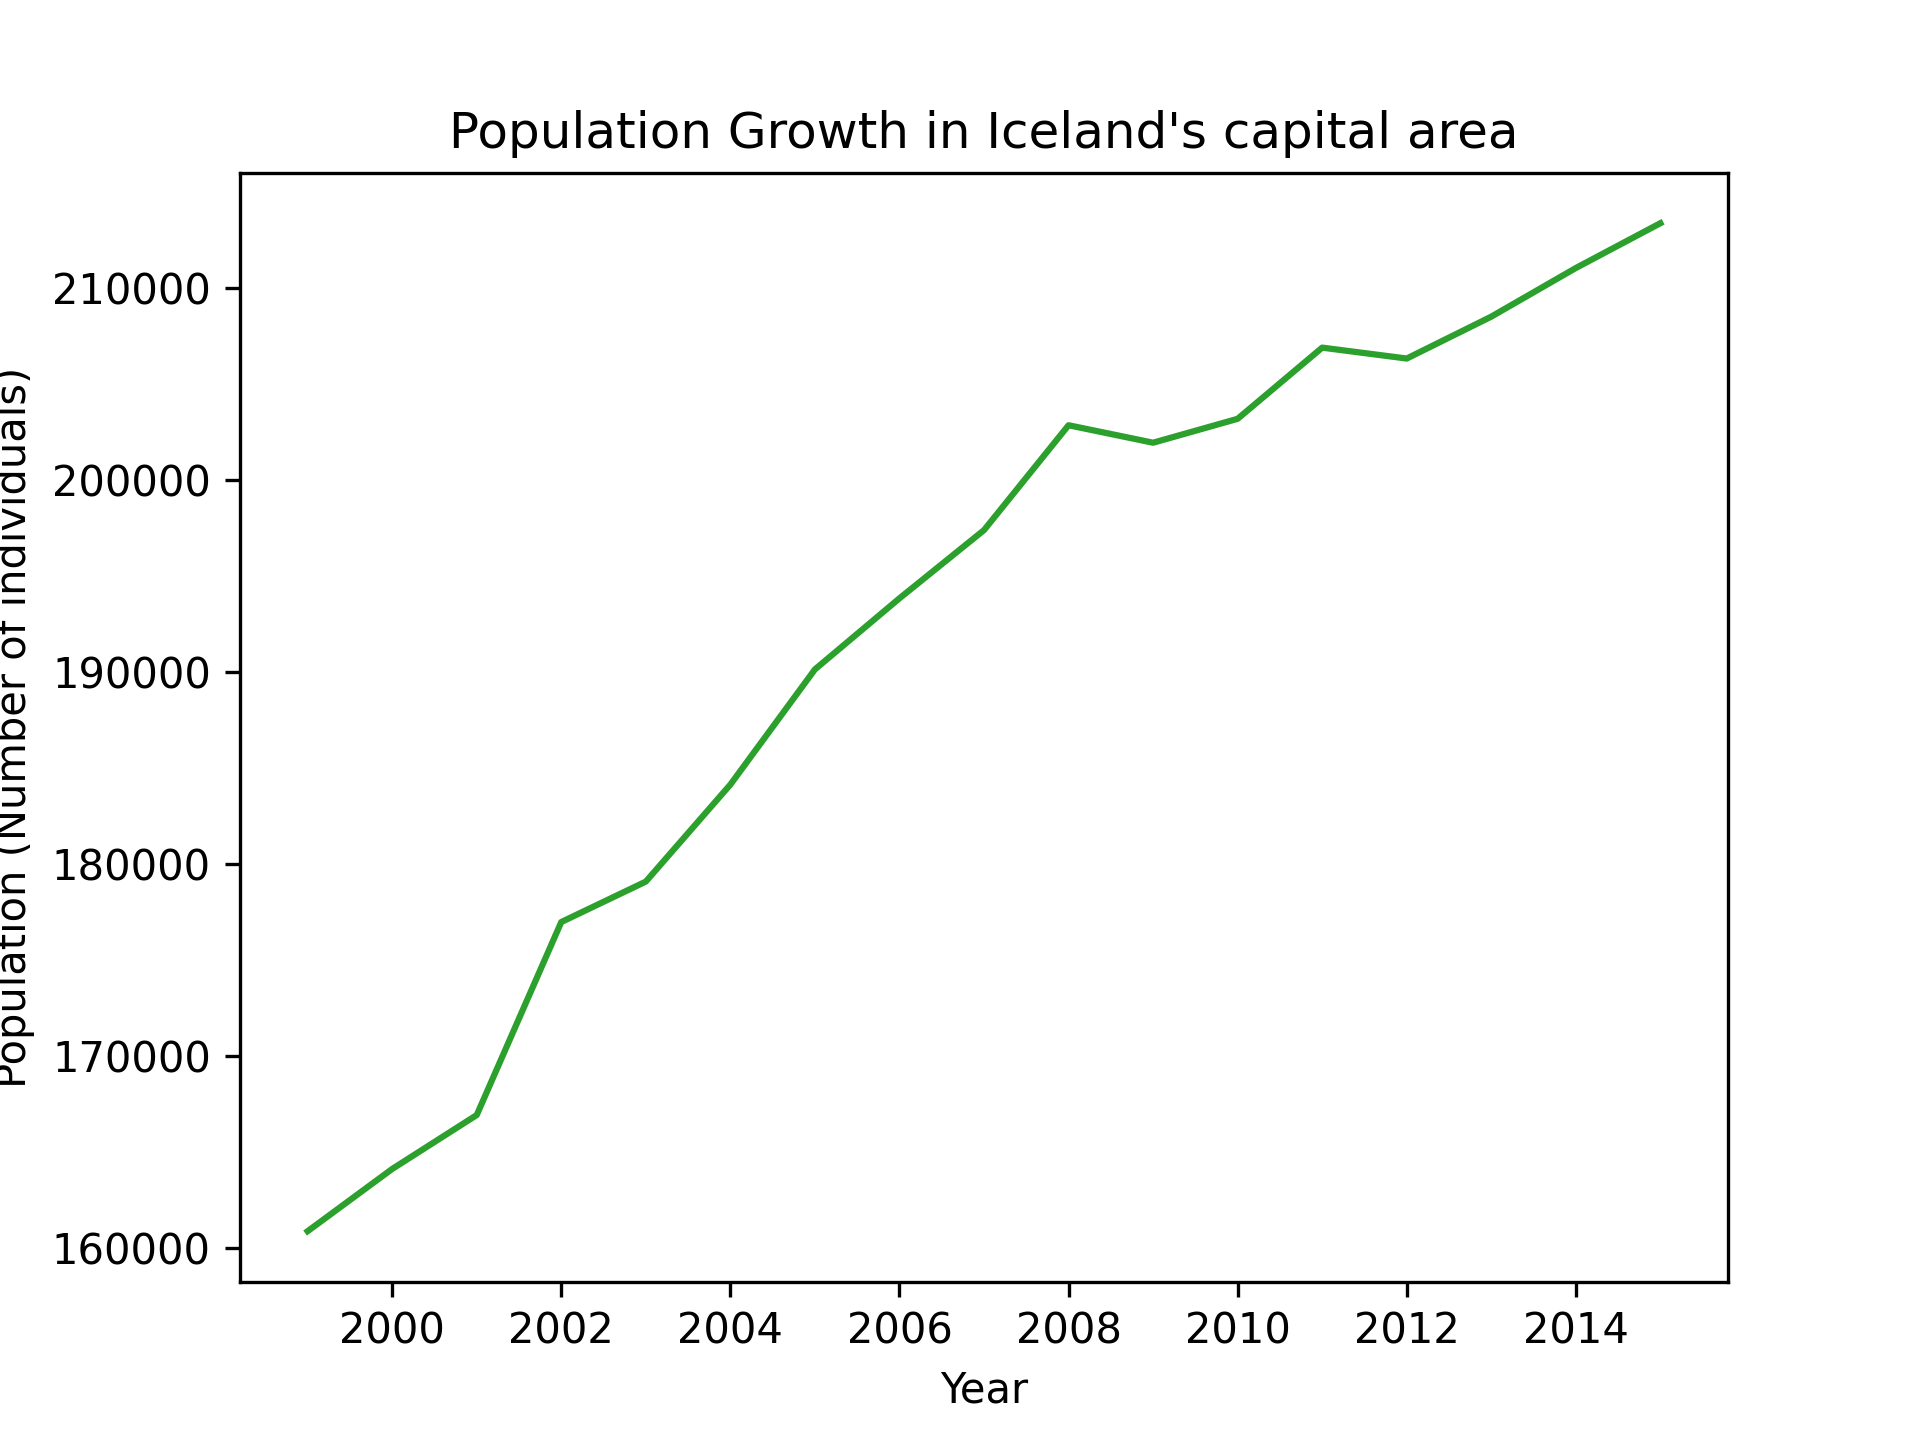
\includegraphics[width=0.8\textwidth]{../figures/population-growth.png}
    \caption{Population trends}
    \label{fig:population-trends}
\end{figure}

The trends show that the water demand and population growth are increasing linearly over time, with some noise in the data, especially in the data for hot water.

The models used in this study are XGBoostRegressor and RandomForestRegressor, since they can handle small datasets and are good at predicting time series data.

\newpage


\section{Results}

The results of the models are shown in Table \ref{tab:results}. The validation accuracy represents the model's performance on unseen data during the validation phase. It is a measure of how well the model predicts outcomes compared to the actual values (the highest value is 1). The MSE, RMSE, and MAE are common metrics used to evaluate regression models. The MSE calculates the average squared difference between predicted and actual values, the RMSE is the square root of the MSE, and the MAE measures the average absolute difference between predicted and actual values. The lower the values of these metrics, the better the model.

\begin{table}[!ht]
    \centering
    \begin{tabular}{llll}
        \hline
        ~                   & hot water model & cold water model & population model \\ \hline
        validation accuracy & 0.76            & 0.91             & 0.96             \\
        MSE                 & 0.22            & 0.12             & 0.01             \\
        RMSE                & 0.47            & 0.34             & 0.06             \\
        MAE                 & 0.42            & 0.32             & 0.05             \\ \hline
    \end{tabular}
    \caption{Results}
    \label{tab:results}
\end{table}

The results show that the models are able to predict water demand and population growth with reasonable accuracy. The models for cold water and population growth perform better than the model for hot water. This is likely due to the noise in the data for hot water, as shown in Figure \ref{fig:water-demand-trends}.

Plotting the predictions against the actual values shows that the models are able to capture the trends in the data, as shown in Figure \ref{fig:water-demand-predictions} and Figure \ref{fig:population-wredictions}.

\begin{figure}[h]
    \centering
    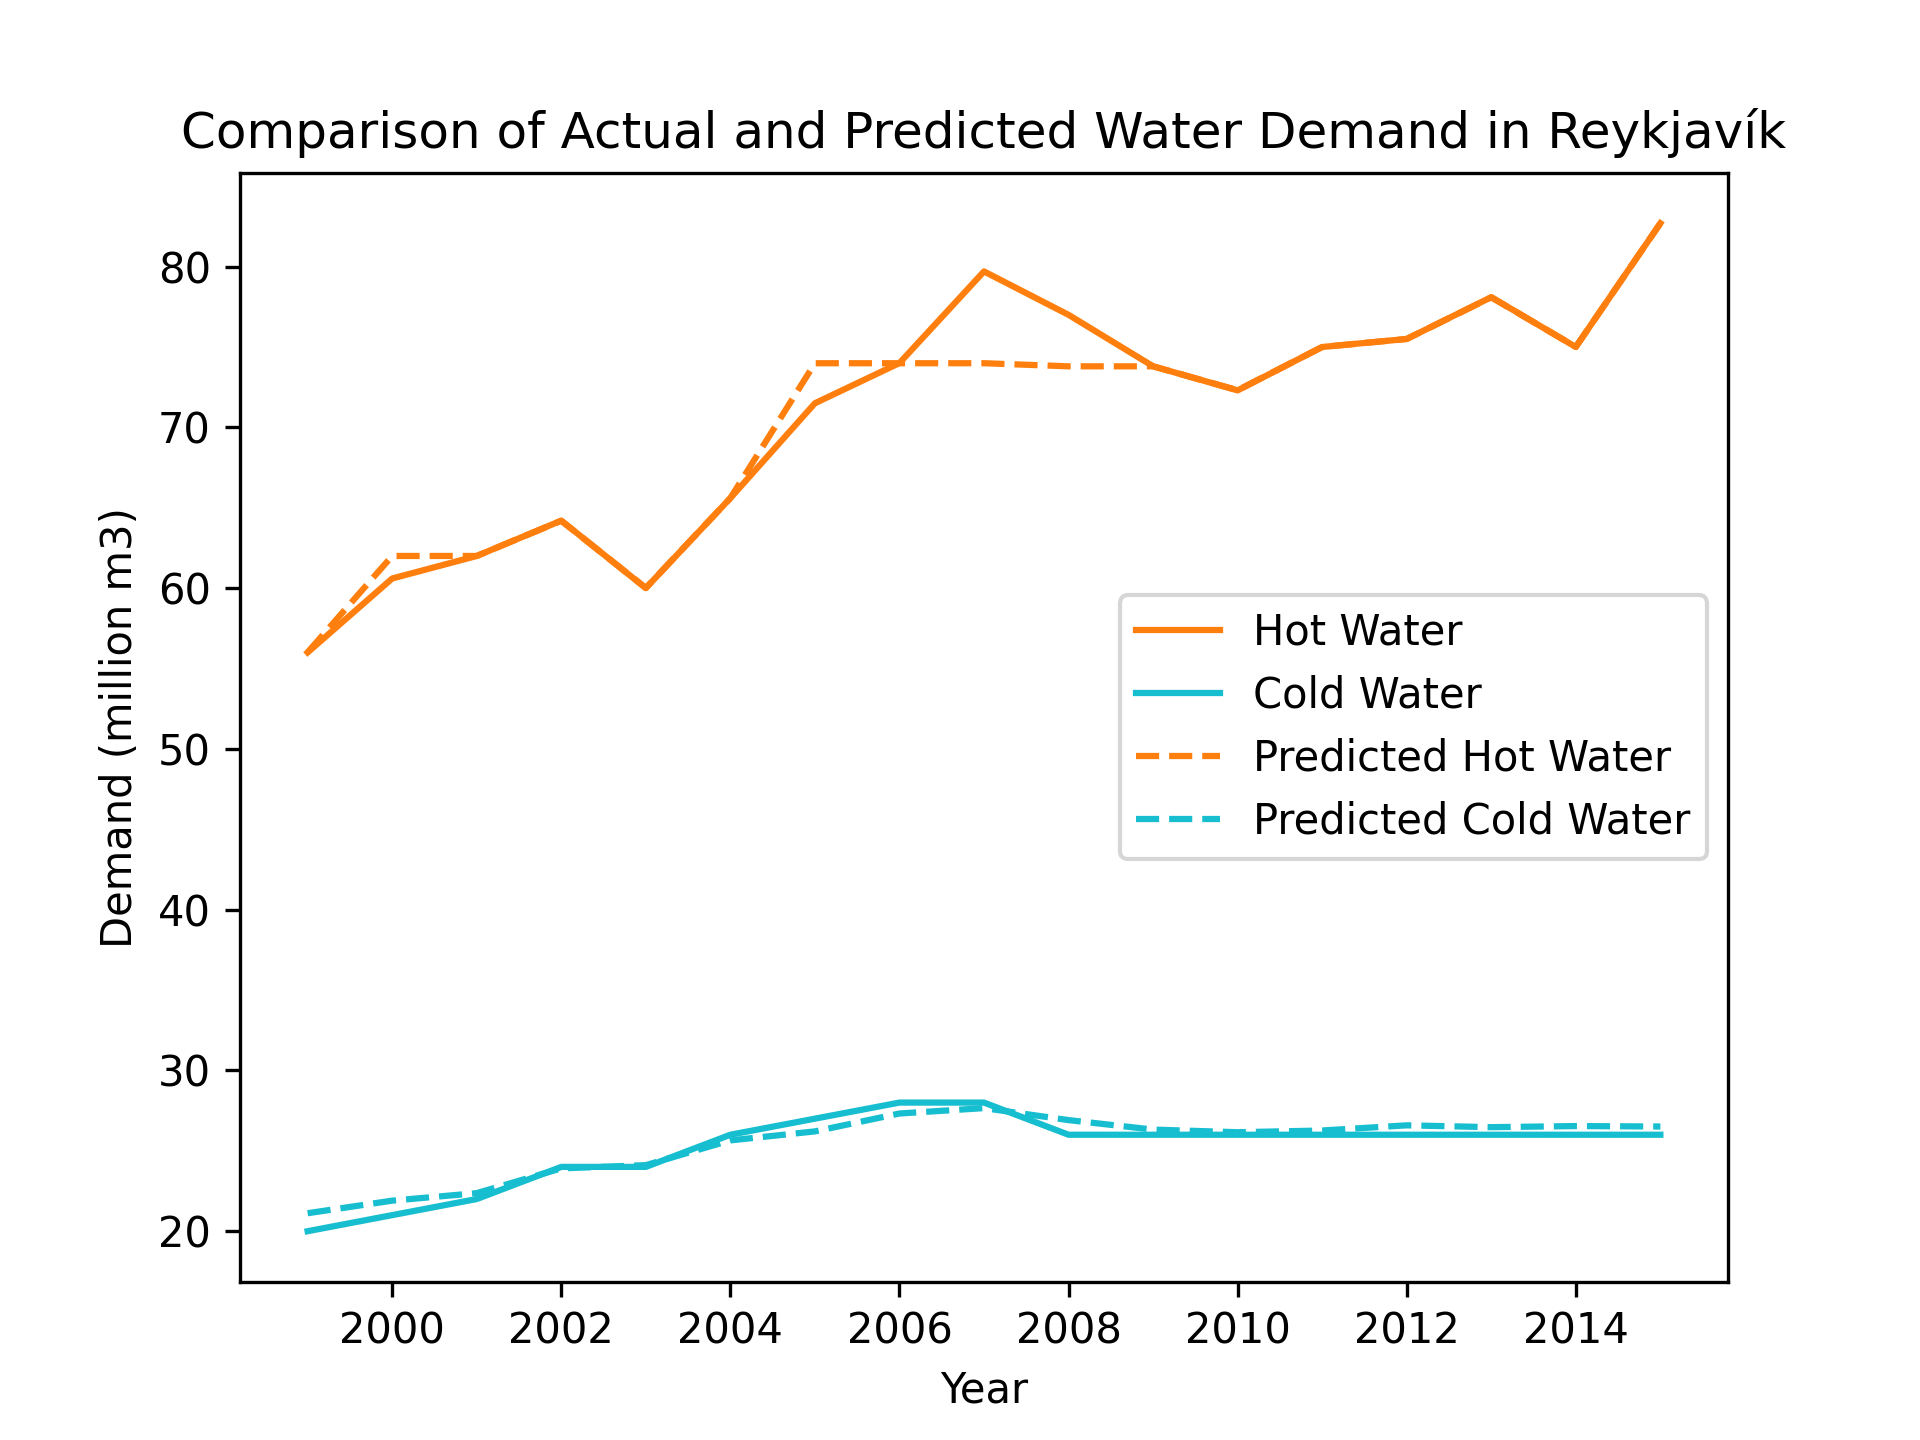
\includegraphics[width=0.8\textwidth]{../figures/comparision-of-actual-and-predicted-water-demand.png}
    \caption{Predictions}
    \label{fig:water-demand-predictions}
\end{figure}

\begin{figure}[h]
    \centering
    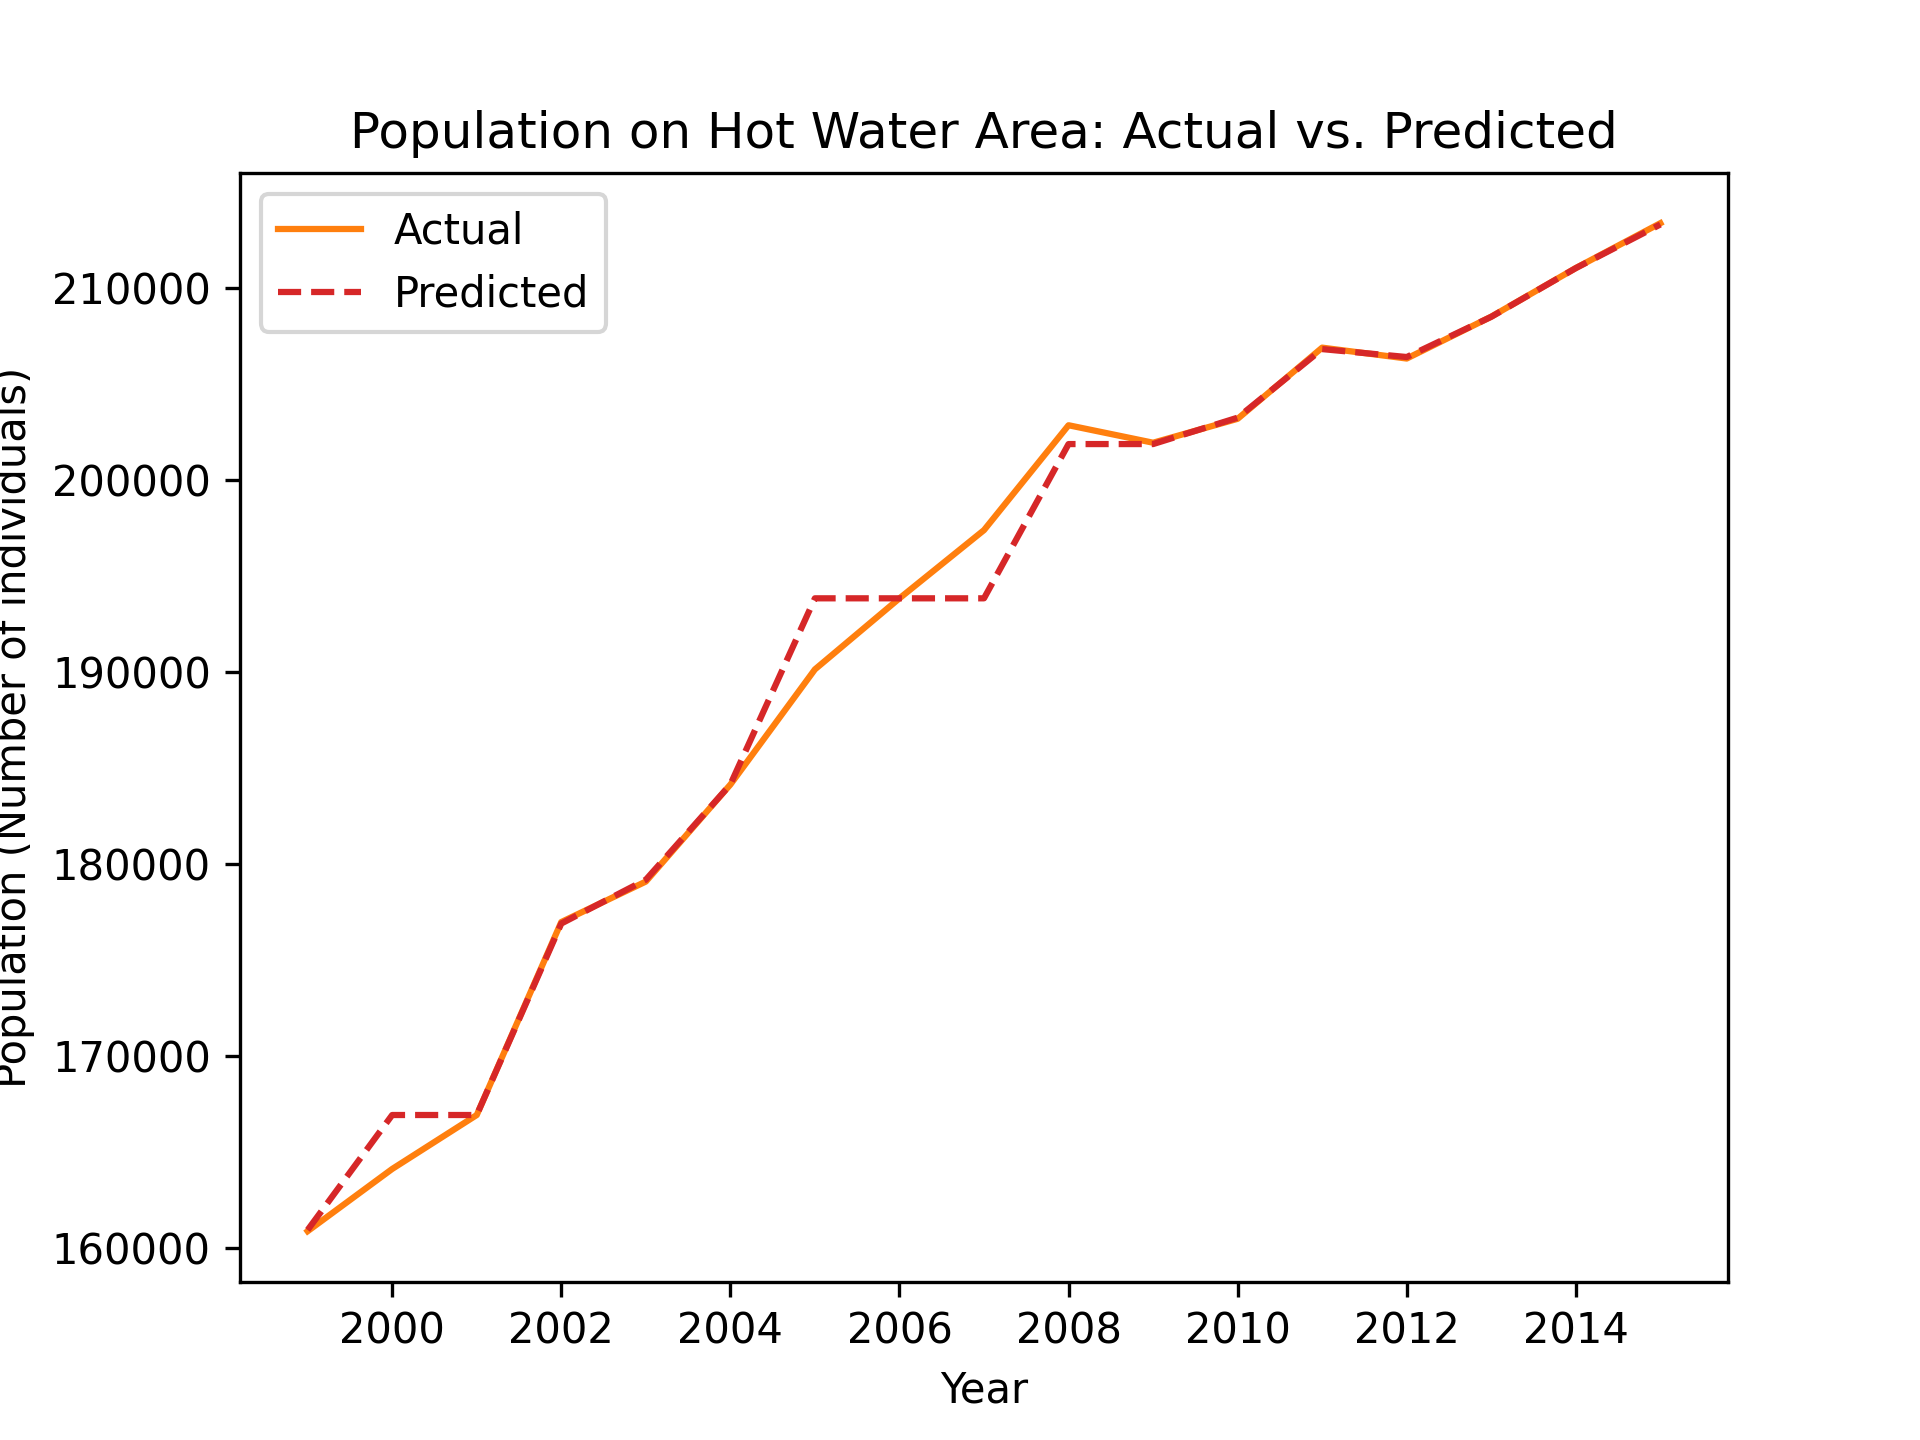
\includegraphics[width=0.8\textwidth]{../figures/population-hot-water-area-actual-vs-predicted.png}
    \caption{Predictions}
    \label{fig:population-wredictions}
\end{figure}

\section{Discussion}

\section{Conclusion}


\bibliographystyle{plain}
\bibliography{mybib}


\end{document}